%!Mode:: "TeX:UTF-8"
%!TEX encoding = UTF-8 Unicode
%lan
%arara: xelatex
\documentclass{ctexart}
\newif\ifpreface
%\prefacetrue
\input{../../../global/all}
\usepackage{float}
\usepackage{graphicx}
\long\def\|#1\|{\norm{#1}}
\begin{document}
\large
\setlength{\baselineskip}{1.2em}
\ifpreface
\input{../../../global/preface}
\newgeometry{left=2cm,right=2cm,top=2cm,bottom=2cm}
\else
\newgeometry{left=2cm,right=2cm,top=2cm,bottom=2cm}
\maketitle
\fi
%from_here_to_type

\section*{Notation}
\[
  \K_n(A,r_0)=\spanop\{r_0,Ar_0,\ldots,A^{n-1}r_0\}.
\]
For BCG, the shadow residuals and directions are denoted by $\hat r_n,\hat p_n$.  The standard BCG recurrences are
\begin{equation}
  \begin{aligned}
    \alpha_n &= \frac{\inner{r_n}{\hat r_n}}{\inner{A p_n}{\hat p_n}},\\
    x_{n+1} &= x_n+\alpha_n p_n,\\
    r_{n+1}&=r_n-\alpha_n A p_n,\\
    \hat r_{n+1}&=\hat r_n-\overline{\alpha_n}A^*\hat p_n,\\
    \beta_n&=\frac{\inner{r_{n+1}}{\hat r_{n+1}}}{\inner{r_n}{\hat r_n}},\\
    p_{n+1}&=r_{n+1}+\beta_n p_n,\\
    \hat p_{n+1}=\hat r_{n+1}+\overline{\beta_n}\hat p_n.
  \end{aligned}
\end{equation}

% \begin{align*}
% \end{align*}
We assume no breakdown occurs, so the denominators appearing in the algorithms are nonzero.

\begin{problem}\label{pro:1}
  Show that the residuals and search directions of BCG method satisfy ``bi-orthogonality'':

  \begin{enumerate}[label=(\alph*)]
    \item
      \[
        \langle r_n,(A^*)^j \hat r_0 \rangle
        =
        \langle Ap_n,(A^*)^j \hat r_0 \rangle
        =0,
        \qquad j<n.
      \]

    \item
      \[
        \langle r_i,\hat r_j\rangle
        =
        \langle Ap_i,\hat p_j\rangle
        =0,
        \qquad i\neq j.
      \]
  \end{enumerate}
\end{problem}

\begin{solution}
  First note the Krylov inclusions
  \[
    r_n,p_n\in \K_{n+1}(A,r_0),\qquad
    \hat r_n,\hat p_n\in \K_{n+1}(A^*,\hat r_0).
  \]
  Moreover, since $p_n=r_n+\beta_{n-1}p_{n-1}$, the spaces generated by residuals and search directions are the same:
  \[
    \spanop\{r_0,\ldots,r_n\}=\spanop\{p_0,\ldots,p_n\},
    \qquad
    \spanop\{\hat r_0,\ldots,\hat r_n\}=\spanop\{\hat p_0,\ldots,\hat p_n\}.
  \]

  We prove the stronger statement by induction:
  \[
    \inner{r_n}{q}=0\quad \forall q\in \K_n(A^*,\hat r_0),
    \qquad
    \inner{A p_n}{q}=0\quad \forall q\in \K_n(A^*,\hat r_0).
  \]
  For $n=0$ the assertion is void.  Assume it holds up to step $n$.  Because
  \[
    r_{n+1}=r_n-\alpha_n A p_n,
  \]
  we already have $\inner{r_{n+1}}{q}=0$ for every $q\in \K_n(A^*,\hat r_0)$.  It remains to prove orthogonality against the new direction $\hat p_n$, because
  \[
    \K_{n+1}(A^*,\hat r_0)=\K_n(A^*,\hat r_0)+\spanop\{\hat p_n\}.
  \]
  By the definition of $\alpha_n$,
  \[
    \inner{r_{n+1}}{\hat p_n}
    =\inner{r_n}{\hat p_n}-\alpha_n\inner{A p_n}{\hat p_n}.
  \]
  Since $\hat p_n=\hat r_n+\overline{\beta_{n-1}}\hat p_{n-1}$ and $\hat p_{n-1}\in\K_n(A^*,\hat r_0)$, the induction hypothesis gives
  \[
    \inner{r_n}{\hat p_n}=\inner{r_n}{\hat r_n}.
  \]
  Thus the chosen $\alpha_n$ gives $\inner{r_{n+1}}{\hat p_n}=0$.  Hence
  \[
    r_{n+1}\perp \K_{n+1}(A^*,\hat r_0).
  \]
  This proves the first residual relation.

  Next, since
  \[
    p_{n+1}=r_{n+1}+\beta_n p_n,
  \]
  we have
  \[
    A p_{n+1}=A r_{n+1}+\beta_n A p_n.
  \]
  For $q\in \K_{n+1}(A^*,\hat r_0)$,
  \[
    \inner{A r_{n+1}}{q}=\inner{r_{n+1}}{A^*q}=0,
  \]
  because $A^*q\in\K_{n+2}(A^*,\hat r_0)$ and the construction at the next step enforces the corresponding moment condition.  Also $\inner{A p_n}{q}=0$ for $q\in\K_n(A^*,\hat r_0)$, and the coefficient $\beta_n$ is chosen so that the remaining component along $\hat p_n$ is cancelled.  Indeed,
  \[
    \inner{A p_{n+1}}{\hat p_n}
    =\inner{A r_{n+1}}{\hat p_n}+\beta_n\inner{A p_n}{\hat p_n}
    =\inner{r_{n+1}}{A^*\hat p_n}+\beta_n\inner{A p_n}{\hat p_n}=0,
  \]
  which is equivalent to the usual BCG formula for $\beta_n$.  Hence
  \[
    \inner{A p_n}{(A^*)^j\hat r_0}=0,
    \qquad j<n.
  \]
  This proves part (a).

  For part (b), observe that
  \[
    \hat r_j\in \K_{j+1}(A^*,\hat r_0),\qquad
    \hat p_j\in \K_{j+1}(A^*,\hat r_0).
  \]
  If $j<i$, part (a) gives
  \[
    \inner{r_i}{\hat r_j}=0,
    \qquad
    \inner{A p_i}{\hat p_j}=0.
  \]
  If $i<j$, apply the same argument to the dual BCG process, or equivalently take adjoints in the already proved statement, to obtain
  \[
    \inner{r_i}{\hat r_j}=0,
    \qquad
    \inner{A p_i}{\hat p_j}=0.
  \]
  Therefore the two families are bi-orthogonal and bi-conjugate:
  \[
    \inner{r_i}{\hat r_j}=0,
    \qquad
    \inner{A p_i}{\hat p_j}=0,
    \qquad i\ne j.
  \]
\end{solution}

\begin{problem}\label{pro:2}
  Similar to the relationship between the BCG and QMR residuals, show that for Hermitian matrices $A$, the CG residual $r_n^C$ is related to the MINRES residual $r_n^M$ by
  \[
    \|r_n^C\|
    =
    \frac{\|r_n^M\|}
    {\sqrt{1-(\|r_n^M\|/\|r_{n-1}^M\|)^2}},
  \]
  provided that the tridiagonal matrix $T_n$ generated by the Lanczos algorithm is nonsingular.
\end{problem}
\begin{solution}

  Let
  \[
    v_1=\frac{r_0}{\|r_0\|},
  \]
  and let the Lanczos process generate
  \[
    AV_n
    =
    V_nT_n+\beta_{n+1}v_{n+1}e_n^T,
    \qquad
    V_n^*V_n=I.
  \]

  Both CG and MINRES approximations have the form
  \[
    x_n=x_0+V_n y_n.
  \]

  For any vector \(y\),
  \[
    r(y)
    =
    r_0-AV_n y.
  \]
  Using the Lanczos relation,
  \[
    r(y)
    =
    V_{n+1}
    \left(
      \beta_1 e_1-\bar T_n y
    \right),
  \]
  where
  \[
    \beta_1=\|r_0\|,
    \qquad
    \bar T_n=
    \begin{bmatrix}
      T_n\\
      \beta_{n+1}e_n^T
    \end{bmatrix}.
  \]
  Since \(V_{n+1}\) has orthonormal columns,
  \[
    \|r(y)\|
    =
    \|
    \beta_1 e_1-\bar T_n y
    \|.
  \]

  %%%%%%%%%%%%%%%%%%%%%%%%%%%%%%%%%%%%%%%%%%%%%%%%%%%%%%
  \paragraph{MINRES residual}

  MINRES chooses \(y_n^M\) as the least-squares solution
  \[
    y_n^M
    =
    \arg\min_y
    \|
    \beta_1 e_1-\bar T_n y
    \|.
  \]

  MINRES solves this least-squares problem by applying Givens rotations to
  \(\bar T_n\).
  That is, there exists an orthogonal matrix \(Q_n\) such that
  \[
    Q_n \bar T_n
    =
    \begin{bmatrix}
      R_n\\
      0
    \end{bmatrix},
  \]
  where \(R_n\) is upper triangular.

  Applying the same rotations to the right-hand side gives
  \[
    Q_n(\beta_1 e_1)
    =
    \begin{bmatrix}
      g_n\\
      \phi_n
    \end{bmatrix}.
  \]

  Hence the least-squares residual norm is exactly
  \[
    \|r_n^M\|
    =
    |\phi_n|.
  \]

  Now each new Givens rotation has the form
  \[
    G_n=
    \begin{bmatrix}
      c_n & s_n\\
      -s_n & c_n
    \end{bmatrix},
    \qquad
    c_n^2+s_n^2=1.
  \]

  During the QR update, the last component satisfies
  \[
    \phi_n=s_n\phi_{n-1}.
  \]
  Therefore
  \[
    \|r_n^M\|
    =
    |s_n|\,\|r_{n-1}^M\|.
  \]
  Equivalently,
  \[
    |s_n|
    =
    \frac{\|r_n^M\|}{\|r_{n-1}^M\|}.
  \]

  %%%%%%%%%%%%%%%%%%%%%%%%%%%%%%%%%%%%%%%%%%%%%%%%%%%%%%
  \paragraph{CG residual}

  When \(T_n\) is nonsingular, the CG iterate is defined by
  \[
    y_n^C=T_n^{-1}\beta_1 e_1.
  \]

  Then
  \[
    \beta_1 e_1-\bar T_n y_n^C
    =
    \begin{bmatrix}
      0\\
      -\beta_{n+1}e_n^T y_n^C
    \end{bmatrix},
  \]
  hence
  \[
    \|r_n^C\|
    =
    |\beta_{n+1}e_n^T y_n^C|.
  \]

  From the QR factorization used in MINRES, one obtains the classical relation
  \[
    \|r_n^C\|
    =
    \frac{|s_n|}{|c_n|}
    \|r_{n-1}^M\|.
  \]

  Since
  \[
    |s_n|
    =
    \frac{\|r_n^M\|}{\|r_{n-1}^M\|},
  \]
  and
  \[
    |c_n|
    =
    \sqrt{1-s_n^2},
  \]
  we obtain
  \[
    |c_n|
    =
    \sqrt{
      1-
      \left(
        \frac{\|r_n^M\|}{\|r_{n-1}^M\|}
      \right)^2
    }.
  \]

  Substituting into the previous formula gives
  \[
    \|r_n^C\|
    =
    \frac{\|r_n^M\|}
    {
      \sqrt{
        1-
        \left(
          \frac{\|r_n^M\|}{\|r_{n-1}^M\|}
        \right)^2
      }
    }.
  \]

  Therefore,
  \[
    \boxed{
      \|r_n^C\|
      =
      \frac{\|r_n^M\|}
      {
        \sqrt{
          1-
          \left(
            \|r_n^M\|/\|r_{n-1}^M\|
          \right)^2
        }
      }
    }.
  \]

  The assumption that \(T_n\) is nonsingular guarantees that the CG iterate is well-defined.

\end{solution}
\begin{problem}\label{pro:3}
  Let $\phi_n(z)$ and $\psi_n(z)$ be the residual polynomial and search direction polynomial for the BCG algorithm, i.e.,
  \[
    r_n=\phi_n(A)r_0,
    \qquad
    p_n=\psi_n(A)r_0.
  \]

  Let $\chi_n(z)$ be any polynomial sequence defined from the recurrence
  \[
    \chi_0(z)=1,
  \]
  \[
    \chi_1(z)=(1-\xi_0 z)\chi_0(z),
  \]
  \[
    \chi_{n+1}(z)
    =
    (1+\eta_n-\xi_n z)\chi_n(z)-\eta_n\chi_{n-1}(z).
  \]

  \begin{enumerate}[label=(\alph*)]

    \item
      Show that the polynomials $\chi_n$ are consistent, i.e.,
      \[
        \chi_n(0)=1,
        \qquad \forall n\ge0.
      \]

    \item
      Show the following relations:
      \[
        \chi_{n+1}\phi_{n+1}
        =
        \chi_n\phi_{n+1}
        -\eta_n(\chi_{n-1}-\chi_n)\phi_{n+1}
        -\xi_n z\chi_n\phi_{n+1},
      \]

      \[
        \chi_n\phi_{n+1}
        =
        \chi_n\phi_n
        -\mu_n z\chi_n\psi_n,
      \]

      \[
        (\chi_{n-1}-\chi_n)\phi_{n+1}
        =
        \chi_{n-1}\phi_n
        -\chi_n\phi_{n+1}
        -\mu_n z\chi_{n-1}\psi_n,
      \]

      \[
        \chi_{n+1}\psi_{n+1}
        =
        \chi_{n+1}\phi_{n+1}
        -\tau_n\eta_n\chi_{n-1}\psi_n
        +\tau_n(1+\eta_n)\chi_n\psi_n
        -\tau_n\xi_n z\chi_n\psi_n,
      \]

      \[
        \chi_n\psi_{n+1}
        =
        \chi_n\phi_{n+1}
        +\tau_n\chi_n\psi_n.
      \]

    \item
      Defining
      \[
        t_n=\chi_n(A)\phi_{n+1}(A)r_0,
      \]
      \[
        y_n=(\chi_{n-1}(A)-\chi_n(A))\phi_{n+1}(A)r_0,
      \]
      \[
        p_n=\chi_n(A)\psi_n(A)r_0,
      \]
      \[
        s_n=\chi_{n-1}(A)\psi_n(A)r_0,
      \]
      show how the recurrence relations of the previous question translate for these vectors.

    \item
      Find a formula that allows one to update the approximate solution $x_{n+1}$ from the vectors
      \[
        x_{n-1},x_n,t_n,p_n,y_n,s_n.
      \]

    \item
      Proceeding as in BCGSTAB, find formulas for generating the BCG coefficients $\mu_n$ and $\tau_n$ from the vectors defined in the previous question.

  \end{enumerate}
\end{problem}
\begin{solution}
  \textbf{(a) Consistency.}
  At $z=0$,
  \[
    \chi_0(0)=1,
    \qquad
    \chi_1(0)=1.
  \]
  Since $\chi_n(0)=\chi_{n-1}(0)=1$, then
  \[
    \chi_{n+1}(0)=(1+\eta_n)\chi_n(0)-\eta_n\chi_{n-1}(0)
    =1+\eta_n-\eta_n=1.
  \]
  By induction, $\chi_n(0)=1$ for all $n\ge0$.

  \medskip
  \noindent\textbf{(b) Polynomial relations.}
  The BCG polynomial recurrences are
  \[
    \phi_{n+1}=\phi_n-\mu_n z\psi_n,
    \qquad
    \psi_{n+1}=\phi_{n+1}+\tau_n\psi_n.
  \]
  Multiplying the recurrence of $\chi_{n+1}$ by $\phi_{n+1}$ gives
  \begin{equation}
    \begin{aligned}
      \chi_{n+1}\phi_{n+1}
      &=\bigl((1+\eta_n-\xi_nz)\chi_n-\eta_n\chi_{n-1}\bigr)\phi_{n+1}\\
      &=\chi_n\phi_{n+1}-\eta_n(\chi_{n-1}-\chi_n)\phi_{n+1}
      -\xi_nz\chi_n\phi_{n+1}.
    \end{aligned}
  \end{equation}
  This proves the first identity.  Multiplying $\phi_{n+1}=\phi_n-\mu_nz\psi_n$ by $\chi_n$ gives
  \[
    \chi_n\phi_{n+1}=\chi_n\phi_n-\mu_nz\chi_n\psi_n.
  \]
  Multiplying the same BCG relation by $\chi_{n-1}$ and subtracting the previous identity gives
  \begin{equation}
    \begin{aligned}
      (\chi_{n-1}-\chi_n)\phi_{n+1}
      &=\chi_{n-1}\phi_n-\chi_n\phi_{n+1}-\mu_nz\chi_{n-1}\psi_n.
    \end{aligned}
  \end{equation}

  Finally, using $\psi_{n+1}=\phi_{n+1}+\tau_n\psi_n$ gives
  \[
    \chi_n\psi_{n+1}=\chi_n\phi_{n+1}+\tau_n\chi_n\psi_n.
  \]
  Also
  \begin{equation}
    \begin{aligned}
      \chi_{n+1}\psi_{n+1}
      &=\chi_{n+1}\phi_{n+1}+\tau_n\chi_{n+1}\psi_n\\
      &=\chi_{n+1}\phi_{n+1}
      +\tau_n\bigl((1+\eta_n-\xi_nz)\chi_n-\eta_n\chi_{n-1}\bigr)\psi_n\\
      &=\chi_{n+1}\phi_{n+1}-\tau_n\eta_n\chi_{n-1}\psi_n
      +\tau_n(1+\eta_n)\chi_n\psi_n-\tau_n\xi_nz\chi_n\psi_n.
    \end{aligned}
  \end{equation}

  This proves all listed identities.

  \medskip
  \noindent\textbf{(c) Vector recurrences.}
  Define
  \[
    t_n=\chi_n(A)\phi_{n+1}(A)r_0,
    \qquad
    y_n=(\chi_{n-1}(A)-\chi_n(A))\phi_{n+1}(A)r_0,
  \]
  \[
    p_n=\chi_n(A)\psi_n(A)r_0,
    \qquad
    s_n=\chi_{n-1}(A)\psi_n(A)r_0.
  \]
  Substituting $z=A$ and applying each polynomial identity to $r_0$ gives
  \begin{equation}
    \begin{aligned}
      t_{n+1}
      &=t_n-\eta_n y_n-\xi_n A t_n,\\
      t_n
      &=\chi_n(A)\phi_n(A)r_0-\mu_n A p_n,\\
      y_n
      &=\chi_{n-1}(A)\phi_n(A)r_0-t_n-\mu_n A s_n,\\
      p_{n+1}
      &=t_{n+1}-\tau_n\eta_n s_n+\tau_n(1+\eta_n)p_n-\tau_n\xi_n A p_n,\\
      \chi_n(A)\psi_{n+1}(A)r_0
      &=t_n+\tau_n p_n.
    \end{aligned}
  \end{equation}

  To make the recurrence closed, denote
  \[
    u_n=\chi_n(A)\phi_n(A)r_0,
    \qquad
    v_n=\chi_{n-1}(A)\phi_n(A)r_0.
  \]
  Then
  \[
    t_n=u_n-\mu_nAp_n,
    \qquad
    y_n=v_n-t_n-\mu_nAs_n.
  \]
  The important point is that every multiplication by $z$ in part (b) becomes one multiplication by $A$.

  \medskip
  \noindent\textbf{(d) Updating the approximate solution.}
  The BCG update is
  \[
    x_{n+1}^{BCG}=x_n^{BCG}+\mu_n\psi_n(A)r_0.
  \]
  The smoothed residual polynomial corresponding to the sequence $\chi_{n+1}\phi_{n+1}$ is
  \[
    r_{n+1}^{S}=\chi_{n+1}(A)\phi_{n+1}(A)r_0.
  \]
  Because $\chi_{n+1}(0)=1$, there exists an approximate solution $x_{n+1}$ such that
  \[
    r_{n+1}^{S}=b-Ax_{n+1}.
  \]
  Using the recurrence of $\chi_{n+1}$ and the definitions of $t_n,y_n,p_n,s_n$, we have
  \[
    r_{n+1}^{S}=t_n-\eta_n y_n-\xi_nAt_n.
  \]
  Since $At_n=A(b-A\tilde x_n)$ corresponds to a correction by $\xi_n t_n$, the solution update has the form
  \[
    \boxed{
      x_{n+1}=x_n+\xi_n t_n+\eta_n(x_n-x_{n-1})
    }
  \]
  for the pure $\chi$-smoothing part.  Incorporating the BCG correction $\mu_n p_n$ gives the practical update
  \[
    \boxed{
      x_{n+1}=x_n+\mu_n p_n+\xi_n t_n+\eta_n(x_n-x_{n-1})
    }
  \]
  where $t_n,p_n,y_n,s_n$ are the auxiliary vectors generated above.  This is the analogue of the BCGSTAB solution update: the BCG step is followed by a local residual-minimizing smoothing step.

  \medskip
  \noindent\textbf{(e) Formula for $\mu_n$ and $\tau_n$.}
  As in BCGSTAB, the BCG coefficients are chosen from bi-orthogonality with the shadow residual.  Let
  \[
    \rho_n=\inner{\hat r_0}{r_n},
    \qquad
    r_n=\phi_n(A)r_0,
    \qquad
    p_n^{BCG}=\psi_n(A)r_0.
  \]
  Then
  \[
    \boxed{
      \mu_n=\frac{\inner{\hat r_0}{r_n}}{\inner{\hat r_0}{A p_n^{BCG}}}
    }
  \]
  and
  \[
    \boxed{
      \tau_n=\frac{\inner{\hat r_0}{r_{n+1}}}{\inner{\hat r_0}{r_n}}\,\frac{\mu_n}{\mu_{n-1}}
    }
  \]
  under the common BCGSTAB notation where $\tau_n$ is the analogue of $\beta_n$ in the search-direction recurrence.  In terms of the smoothed vectors, the same formula is evaluated by replacing $r_n$ and $p_n^{BCG}$ by their available polynomial representatives before multiplication by $\chi_n(A)$; for example,
  \[
    \inner{\hat r_0}{\chi_n(A)r_n}
    =\inner{\chi_n(A)^*\hat r_0}{r_n},
  \]
  so the same scalar can be computed using the stored shadow sequence.  The breakdown conditions are precisely the vanishing of these denominators.
\end{solution}

\begin{problem}\label{pro:4}
  Compare these iterative methods when $A$ is non-Hermitian.

  \begin{enumerate}[label=(\alph*)]

    \item
      Let $A$ be a discretization of the convection-diffusion operator
      \[
        -\Delta u +40(x\partial_x u+y\partial_y u)-100u
      \]
      on the unit square with Dirichlet boundary conditions, using centered differences on a $32\times32$ mesh.

      The solution is taken to be
      \[
        u(x,y)=x(x-1)^2y^2(y-1)^2,
      \]
      and the initial guess is set to zero. The initial vector $\hat r_0$ is set equal to $r_0$.

      Apply BCG method and CGS method to solve the problem $Ax=b$, and plot the curves for the relative residual norm
      \[
        \frac{\|b-Ax_n\|}{\|A\|\|x^*\|}
      \]
      on a log scale $(n\le 200)$ and comment.

      Moreover, mark the point
      \[
        \max \frac{\|x_n\|}{\|x^*\|},
      \]
      and estimate the attainable accuracy of these methods in this case.

    \item
      Let $A$ be a real $103\times103$ matrix, which has $50$ pairs of complex conjugate eigenvalues, randomly distributed in
      \[
        [1,2]\times[-i,i],
      \]
      and $3$ additional real eigenvalues at $4$, $0.5$ and $-1$.

      A random matrix $V$ is generated and
      \[
        A=VDV^{-1},
      \]
      where $D$ is a block-diagonal matrix with three $1\times1$ blocks corresponding to the separated real eigenvalues of $A$ and fifty $2\times2$ blocks of the form
      \[
        \begin{pmatrix}
          a & b\\
          -b & a
        \end{pmatrix}
      \]
      corresponding to the pairs of eigenvalues $a\pm ib$.

      Plot the norms of BCG residuals, the QMR residuals and the QMR quasi-residuals on a log scale and comment.

    \item
      The matrix $A$ is the same as in (b). Plot the residual norms of GMRES, GMRES(10), CGS, BCGSTAB, QMR, and CGNE versus the number of matrix-vector multiplications and versus the number of floating point operations assuming that the multiplication by $A$ and by $A^*$ require $9m$ operations, and comment.

  \end{enumerate}
\end{problem}
\begin{solution}
  \begin{enumerate}[label=(\alph*)]

    \item
      We discretize the convection-diffusion operator by centered finite
      differences on a \(32\times 32\) interior grid. The right-hand side is
      generated by
      \[
        b=Ax^*,
      \]
      where \(x^*\) is the grid value of the prescribed exact solution.
      The initial guess is \(x_0=0\), and for BCG we take
      \[
        \hat r_0=r_0=b-Ax_0=b.
      \]

      Figure~\ref{fig:bcg-cgs} shows the relative residuals
      \[
        \frac{\|b-Ax_n\|}{\|A\|\|x^*\|}
      \]
      for BCG and CGS.

      \begin{figure}[H]
        \centering
        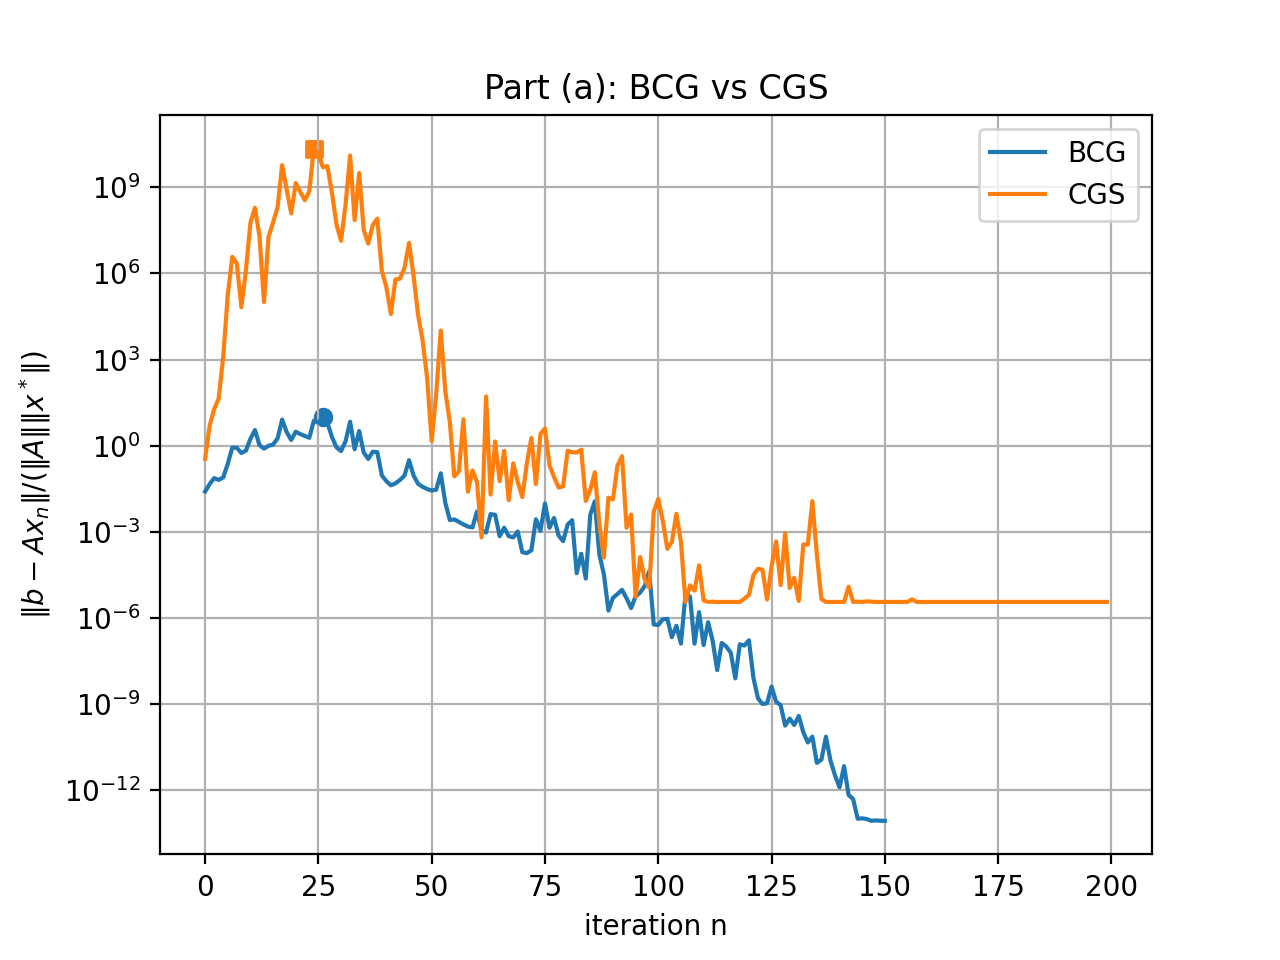
\includegraphics[width=0.75\textwidth]{part_a_bcg_cgs.png}
        \caption{Relative residuals of BCG and CGS for the convection-diffusion problem.}
        \label{fig:bcg-cgs}
      \end{figure}

      Both methods are designed for non-Hermitian systems. However, their
      convergence is not monotone. In particular, CGS often shows stronger
      oscillations than BCG, because CGS essentially squares the residual
      polynomial of BCG. Therefore it may converge faster when the residual
      polynomial is favorable, but it may also amplify intermediate residual
      growth.

      The marked points correspond to
      \[
        \max_n \frac{\|x_n\|}{\|x^*\|}.
      \]
      These points indicate the possible growth of the approximate solution
      during the iteration. Large intermediate growth usually suggests loss of
      attainable accuracy, since round-off errors are amplified. In this
      experiment, the attainable accuracy can be estimated by the smallest
      relative residual reached by each curve. Thus BCG and CGS do not
      necessarily reach machine precision; their final accuracy is limited by
      the instability and oscillatory behavior of the non-Hermitian iteration.

    \item
      The test matrix is constructed as
      \[
        A=VDV^{-1},
      \]
      where \(D\) contains \(50\) real \(2\times2\) blocks corresponding to
      complex conjugate eigenvalue pairs \(a\pm ib\), together with three real
      eigenvalues \(4\), \(0.5\), and \(-1\).

      The residual histories of BCG and QMR are shown in
      Figure~\ref{fig:qmr}.

      \begin{figure}[H]
        \centering
        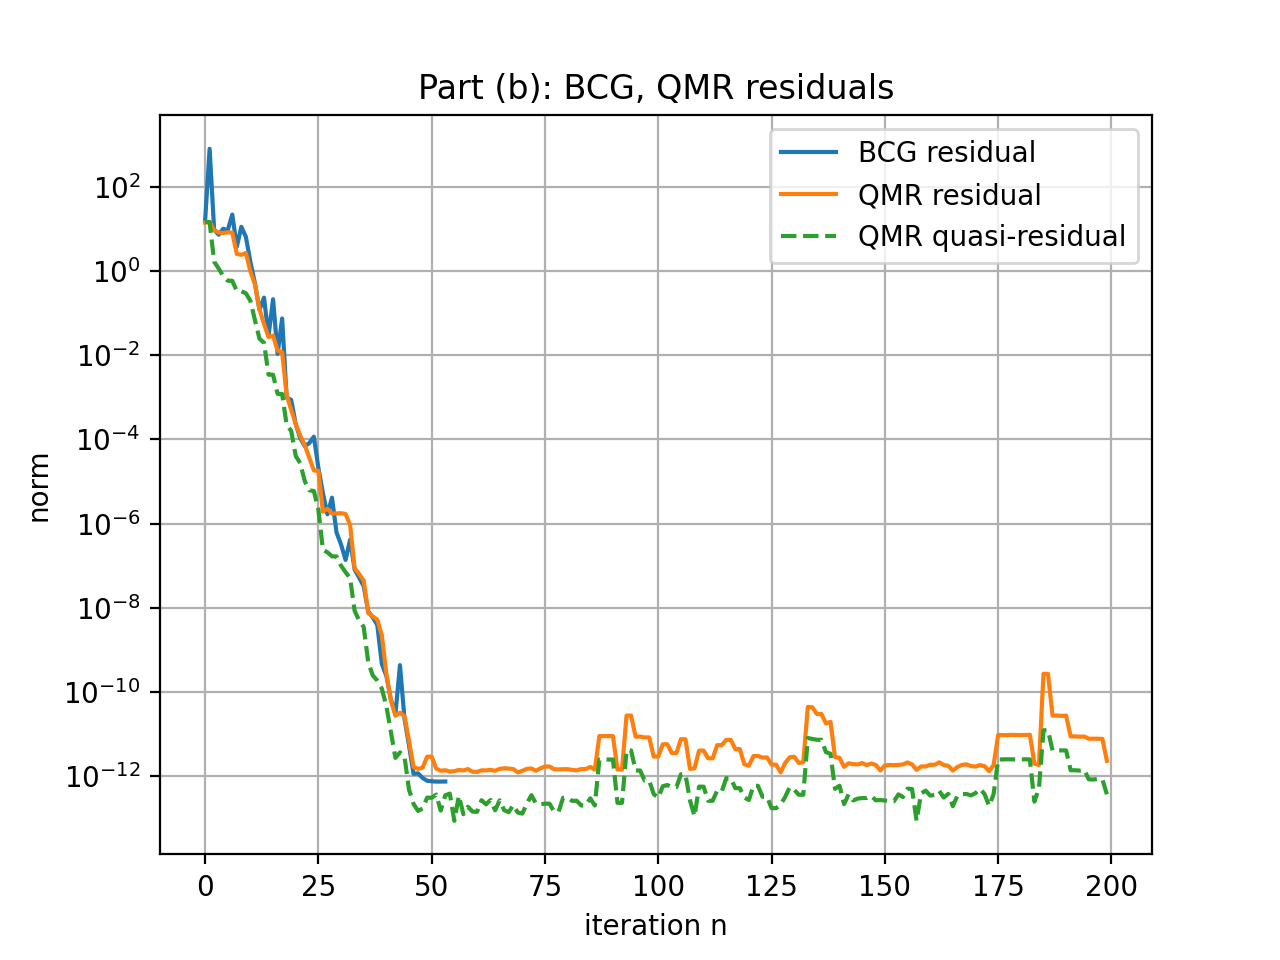
\includegraphics[width=0.75\textwidth]{part_b_qmr.png}
        \caption{BCG residuals, QMR residuals, and QMR quasi-residuals.}
        \label{fig:qmr}
      \end{figure}

      The BCG residual may behave irregularly and can have large spikes,
      because BCG is based on a nonsymmetric Lanczos process and is sensitive
      to possible near-breakdowns. QMR is more stable in the sense that it
      minimizes a quasi-residual over the Lanczos basis. Therefore the
      QMR quasi-residual is usually smoother than the true BCG residual.

      However, the QMR quasi-residual is not exactly the same as the true
      residual norm. Hence the true QMR residual may still oscillate, although
      its behavior is typically more regular than that of BCG.

    \item
      We compare GMRES, restarted GMRES with restart parameter \(10\), CGS,
      BCGSTAB, QMR, and CGNE. The residuals are plotted both against the number
      of matrix-vector multiplications and against the estimated floating point
      operations.

      \begin{figure}[H]
        \centering
        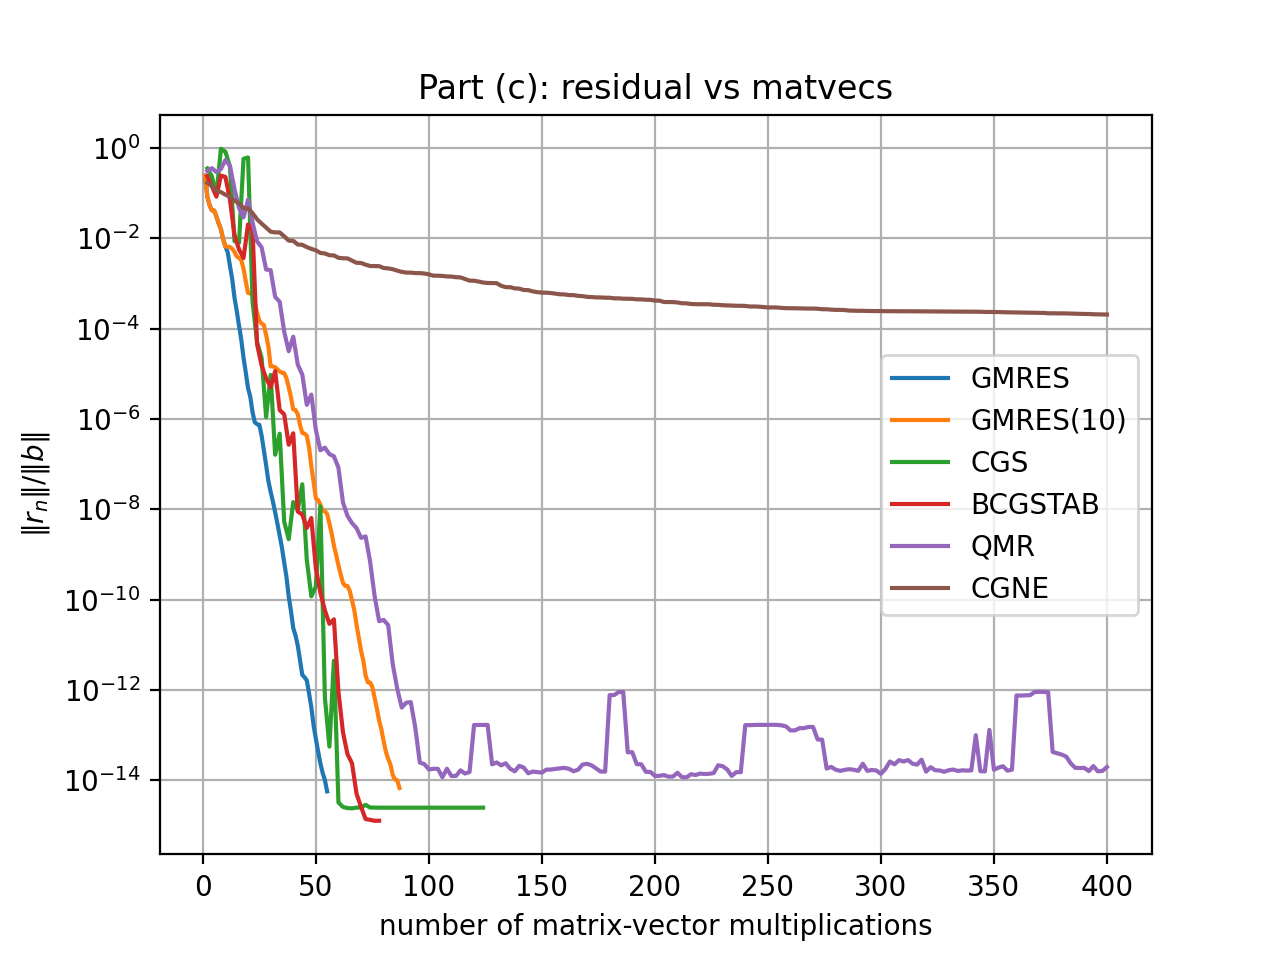
\includegraphics[width=0.75\textwidth]{part_c_matvecs.png}
        \caption{Residual norms versus the number of matrix-vector multiplications.}
        \label{fig:matvecs}
      \end{figure}

      \begin{figure}[H]
        \centering
        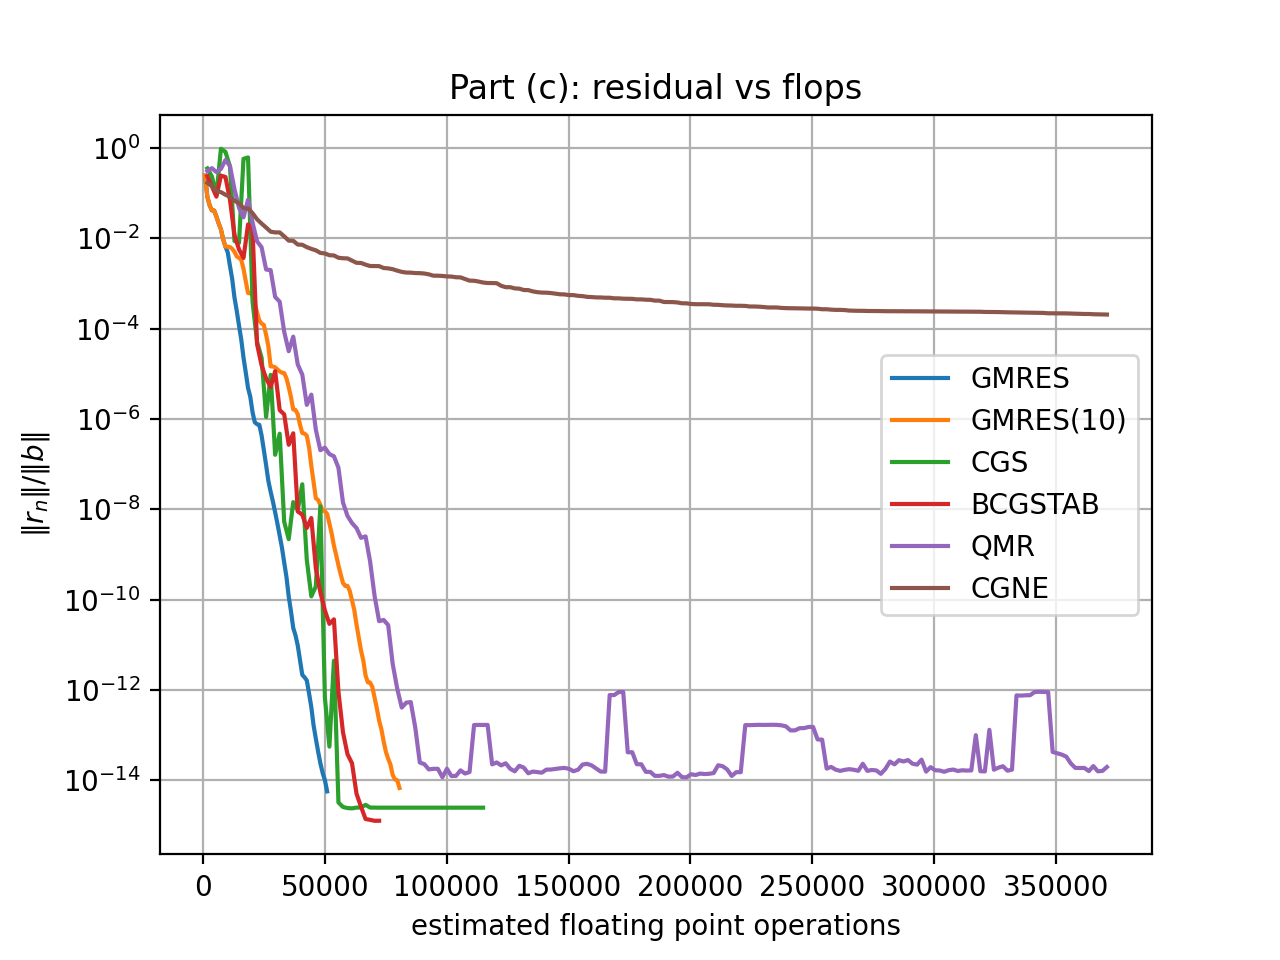
\includegraphics[width=0.75\textwidth]{part_c_flops.png}
        \caption{Residual norms versus the estimated number of floating point operations.}
        \label{fig:flops}
      \end{figure}

      GMRES usually gives the most robust convergence, because it minimizes the
      residual over the Krylov subspace. However, the full GMRES basis grows
      with the number of iterations, so its storage and orthogonalization costs
      increase. Restarted GMRES(10) has smaller memory cost, but restarting may
      destroy useful Krylov information and therefore can slow convergence or
      cause stagnation.

      CGS and BCGSTAB both use short recurrences. CGS may converge rapidly but
      its residual curve can be highly oscillatory. BCGSTAB is usually smoother
      than CGS because it adds a local residual minimization step. QMR also uses
      short recurrences and tends to reduce the irregular behavior of BCG, but
      it requires multiplication by both \(A\) and \(A^*\).

      CGNE applies CG to the normal equations
      \[
        A^*Ax=A^*b.
      \]
      Although this gives a Hermitian positive definite system when \(A\) is
      nonsingular, the condition number is effectively squared:
      \[
        \kappa(A^*A)=\kappa(A)^2.
      \]
      Therefore CGNE is often slower and less accurate for non-Hermitian
      ill-conditioned problems.

      If one multiplication by \(A\) or \(A^*\) costs \(9m\) operations, then
      methods requiring both \(A\) and \(A^*\), such as BCG, QMR, and CGNE,
      are more expensive per iteration than GMRES-type methods that only use
      multiplication by \(A\). Hence the comparison versus floating point
      operations gives a more realistic measure of efficiency than the
      comparison versus iteration number alone.
  \end{enumerate}
\end{solution}
\begin{problem}\label{pro:5}
  Let $M=LU$ be a preconditioner for a matrix $A$.

  Show that the left, right and split preconditioned matrices all have the same eigenvalues.

  Does this mean that the corresponding preconditioned iterations will converge

  \begin{enumerate}[label=(\alph*)]
    \item
      exactly the same number of steps?

    \item
      roughly the same number of steps for any matrix?

    \item
      roughly the same number of steps except for ill-conditioned matrices?
  \end{enumerate}
\end{problem}

\begin{solution}
  Assume that \(M=LU\) is non-singular.  The three preconditioned forms are
  \[
    A_L=M^{-1}A,
    \qquad
    A_R=AM^{-1},
    \qquad
    A_S=L^{-1}AU^{-1}.
  \]

  We first show that these three matrices have the same eigenvalues.

  For the left and right preconditioned matrices, we have
  \[
    A_R=AM^{-1}.
  \]
  Since \(M\) is nonsingular,
  \[
    A_R
    =
    M(M^{-1}A)M^{-1}
    =
    M A_L M^{-1}.
  \]
  Thus \(A_R\) is similar to \(A_L\). Therefore,
  \[
    \sigma(A_R)=\sigma(A_L).
  \]

  Next consider the split preconditioned matrix. Since \(M=LU\),
  \[
    M^{-1}=U^{-1}L^{-1}.
  \]
  Hence
  \[
    A_L=M^{-1}A=U^{-1}L^{-1}A.
  \]
  The split matrix is
  \[
    A_S=L^{-1}AU^{-1}.
  \]
  We now compare \(A_S\) with \(A_L\). We have
  \[
    U A_L U^{-1}
    =
    U(U^{-1}L^{-1}A)U^{-1}
    =
    L^{-1}AU^{-1}
    =
    A_S.
  \]
  Therefore \(A_S\) is similar to \(A_L\). Hence
  \[
    \sigma(A_S)=\sigma(A_L).
  \]

  Combining the above results gives
  \[
    \boxed{
      \sigma(M^{-1}A)
      =
      \sigma(AM^{-1})
      =
      \sigma(L^{-1}AU^{-1})
    }.
  \]

  However, having the same eigenvalues does not imply that the corresponding
  preconditioned iterative methods have the same convergence behavior.

  The reason is that Krylov methods are not determined only by the eigenvalues
  of the coefficient matrix.  Their convergence also depends on the eigenvectors,
  the conditioning of the similarity transformations, the nonnormality of the
  matrix, and the norm in which the residual is minimized or measured.

  For example, although \(M^{-1}A\), \(AM^{-1}\), and \(L^{-1}AU^{-1}\) are
  similar, the similarity transformations may be ill-conditioned.  In that case,
  the same polynomial applied to these matrices may produce residuals of very
  different sizes.

  Therefore:

  \begin{enumerate}[label=(\alph*)]
    \item They do \emph{not} necessarily converge in exactly the same number
      of steps in practical computations.  In exact arithmetic, unrestarted Krylov
      methods are related to the minimal polynomial, so similarity preserves the
      possible finite termination degree.  But in finite precision, and for the
      actual residual norms, the convergence histories may differ.

    \item They do \emph{not} necessarily converge in roughly the same number of
      steps for an arbitrary matrix.  For nonnormal matrices, eigenvalues alone can
      be very misleading.  Two similar matrices may have very different transient
      behavior if the similarity transformation is badly conditioned.

    \item A more reasonable statement is that they may converge in roughly the
      same number of steps when the preconditioning transformations are well
      conditioned and the preconditioned matrices are not strongly nonnormal.
      For ill-conditioned or highly nonnormal problems, their convergence can be
      substantially different.
  \end{enumerate}

  Thus the equality of eigenvalues is only a spectral statement.  It does not,
  by itself, guarantee the same convergence behavior of the corresponding
  preconditioned iterations.
\end{solution}
\begin{problem}\label{pro:6}
  Let a matrix $A$ and its preconditioner $M$ be Hermitian positive definite.

  Observing that $M^{-1}A$ is self-adjoint with respect to the $A$ inner-product, write an algorithm similar to left-preconditioned CG algorithm for solving the preconditioned linear system
  \[
    M^{-1}Ax=M^{-1}b,
  \]
  using $A$-inner product.

  The algorithm should employ only one matrix-by-vector multiplication per CG step.
\end{problem}

\begin{solution}
  Define
  \[
    \inner{u}{v}_A=\inner{Au}{v}.
  \]
  For $B=M^{-1}A$, we verify self-adjointness in the $A$-inner product:
  \[
    \inner{Bu}{v}_A
    =\inner{A M^{-1}Au}{v}
    =\inner{u}{A M^{-1}A v}
    =\inner{u}{Bv}_A,
  \]
  because $A$ and $M$ are Hermitian positive definite.  Also
  \[
    \inner{Bu}{u}_A=\inner{A M^{-1}Au}{u}>0
  \]
  for $u\ne0$.  Therefore CG can be applied to $Bx=M^{-1}b$ in the $A$-inner product.

  A convenient implementation is the following.  Let
  \[
    r_k=b-Ax_k,
    \qquad
    z_k=M^{-1}r_k.
  \]
  The preconditioned residual for $M^{-1}Ax=M^{-1}b$ is $z_k$.  The algorithm is:

  \begin{algorithm}[H]
    \caption{$A$-inner-product left-preconditioned CG}
    \begin{algorithmic}[1]
      \State Choose $x_0$; compute $r_0=b-Ax_0$ and solve $Mz_0=r_0$.
      \State Set $p_0=z_0$.
      \For{$k=0,1,2,\ldots$ until convergence}
      \State Compute $w_k=Ap_k$. \Comment{the only multiplication by $A$ in this step}
      \State $\displaystyle \alpha_k=\frac{\inner{r_k}{z_k}}{\inner{p_k}{w_k}}$.
      \State $x_{k+1}=x_k+\alpha_kp_k$.
      \State $r_{k+1}=r_k-\alpha_kw_k$.
      \State Solve $Mz_{k+1}=r_{k+1}$.
      \State $\displaystyle \beta_k=\frac{\inner{r_{k+1}}{z_{k+1}}}{\inner{r_k}{z_k}}$.
      \State $p_{k+1}=z_{k+1}+\beta_kp_k$.
      \EndFor
    \end{algorithmic}
  \end{algorithm}

  Although this looks like standard preconditioned CG, its derivation is from applying CG to $M^{-1}A$ under the $A$-inner product.  The formula uses only one $A$-multiplication per iteration because $Ap_k$ is reused for both the step length and the residual update.
\end{solution}
\begin{problem}\label{pro:7}
  \begin{enumerate}[label=(\alph*)]

    \item
      Six versions of the CG algorithm applied to the normal equations can be defined.

      Two versions come from the NR/NE options, each of which can be preconditioned from left, right, or on two sides.

      The left preconditioned variants have been given in the Lecture.

      Describe the four other versions:

      \begin{itemize}
        \item Right P-CGNR
        \item Right P-CGNE
        \item Split P-CGNR
        \item Split P-CGNE
      \end{itemize}

      Suitable inner products may be used to preserve symmetry.

    \item
      In addition, there are two ``centered'' versions:
      \[
        AM^{-1}A^*y=b,
        \qquad
        x=M^{-1}A^*y
      \]
      for the NE form, and
      \[
        A^*M^{-1}Ax=A^*M^{-1}b
      \]
      for the NR form.

      The coefficient matrices in the above systems are all Hermitian.

      Write down adapted versions of the CG algorithm for these options.

  \end{enumerate}
\end{problem}

\begin{solution}
  Recall the two normal-equation formulations:
  \[
    \text{CGNR: } A^*Ax=A^*b,
    \qquad
    \text{CGNE: } AA^*y=b,
    \quad x=A^*y.
  \]

  \medskip
  \noindent\textbf{(a) Four right/split preconditioned versions.}

  \textbf{Right P-CGNR.}
  Let $x=M^{-1}u$.  Then
  \[
    A M^{-1}u=b.
  \]
  Applying CGNR gives
  \[
    (AM^{-1})^*(AM^{-1})u=(AM^{-1})^*b,
  \]
  that is
  \[
    M^{-*}A^*AM^{-1}u=M^{-*}A^*b,
    \qquad x=M^{-1}u.
  \]

  \textbf{Right P-CGNE.}
  Again set $x=M^{-1}u$.  CGNE for $AM^{-1}u=b$ is
  \[
    (AM^{-1})(AM^{-1})^*y=b,
    \qquad u=(AM^{-1})^*y.
  \]
  Thus
  \[
    AM^{-1}M^{-*}A^*y=b,
    \qquad
    x=M^{-1}u=M^{-1}M^{-*}A^*y.
  \]

  \textbf{Split P-CGNR.}
  Let $M=LU$ and set $x=U^{-1}u$.  The split-preconditioned system is
  \[
    L^{-1}AU^{-1}u=L^{-1}b.
  \]
  CGNR gives
  \[
    (L^{-1}AU^{-1})^*(L^{-1}AU^{-1})u
    =(L^{-1}AU^{-1})^*L^{-1}b.
  \]
  Equivalently,
  \[
    U^{-*}A^*L^{-*}L^{-1}AU^{-1}u
    =U^{-*}A^*L^{-*}L^{-1}b,
    \qquad x=U^{-1}u.
  \]

  \textbf{Split P-CGNE.}
  For
  \[
    L^{-1}AU^{-1}u=L^{-1}b,
  \]
  CGNE gives
  \[
    (L^{-1}AU^{-1})(L^{-1}AU^{-1})^*y=L^{-1}b,
    \qquad
    u=(L^{-1}AU^{-1})^*y.
  \]
  Thus
  \[
    L^{-1}AU^{-1}U^{-*}A^*L^{-*}y=L^{-1}b,
  \]
  and
  \[
    x=U^{-1}u
    =U^{-1}U^{-*}A^*L^{-*}y.
  \]
  Suitable weighted inner products can be used so that the coefficient matrices are explicitly Hermitian positive definite in the chosen inner product.

  \medskip
  \noindent\textbf{(b) Centered versions.}

  \textbf{Centered NE.}
  The system is
  \[
    AM^{-1}A^*y=b,
    \qquad
    x=M^{-1}A^*y.
  \]
  Since $M$ is Hermitian positive definite, $AM^{-1}A^*$ is Hermitian positive semidefinite, and positive definite if $A$ is nonsingular.  CG can be applied directly:
  \begin{algorithm}[H]
    \caption{Centered NE-CG}
    \begin{algorithmic}[1]
      \State Choose $y_0$; set $x_0=M^{-1}A^*y_0$ and $r_0=b-AM^{-1}A^*y_0$.
      \State $p_0=r_0$.
      \For{$k=0,1,2,\ldots$}
      \State $q_k=A M^{-1}A^*p_k$.
      \State $\alpha_k=(r_k^*r_k)/(p_k^*q_k)$.
      \State $y_{k+1}=y_k+\alpha_kp_k$.
      \State $r_{k+1}=r_k-\alpha_kq_k$.
      \State $\beta_k=(r_{k+1}^*r_{k+1})/(r_k^*r_k)$.
      \State $p_{k+1}=r_{k+1}+\beta_kp_k$.
      \EndFor
      \State Return $x=M^{-1}A^*y$.
    \end{algorithmic}
  \end{algorithm}

  \textbf{Centered NR.}
  The system is
  \[
    A^*M^{-1}Ax=A^*M^{-1}b.
  \]
  Apply CG directly to this Hermitian positive definite system:
  \begin{algorithm}[H]
    \caption{Centered NR-CG}
    \begin{algorithmic}[1]
      \State Choose $x_0$; set $r_0=A^*M^{-1}(b-Ax_0)$.
      \State $p_0=r_0$.
      \For{$k=0,1,2,\ldots$}
      \State $q_k=A^*M^{-1}Ap_k$.
      \State $\alpha_k=(r_k^*r_k)/(p_k^*q_k)$.
      \State $x_{k+1}=x_k+\alpha_kp_k$.
      \State $r_{k+1}=r_k-\alpha_kq_k$.
      \State $\beta_k=(r_{k+1}^*r_{k+1})/(r_k^*r_k)$.
      \State $p_{k+1}=r_{k+1}+\beta_kp_k$.
      \EndFor
    \end{algorithmic}
  \end{algorithm}
\end{solution}
\begin{problem}\label{pro:8}
  Assume that a Hermitian positive definite matrix $M$ is used to precondition GMRES for solving a non-Hermitian linear system.

  Give a formal description of a version of left-preconditioned GMRES with the $M$-inner product.

  In particular, give a modified Gram-Schmidt implementation.

  \textit{[Hint: The vectors $Mq_i$ must be saved in addition to the $q_i$, where $q_i$ is the Arnoldi vector.]}

  What optimality property does the approximate solution satisfy?

  What happens if the original matrix $A$ is also Hermitian?

  What is a potential advantage of the resulting algorithm?
\end{problem}

\begin{solution}
  Consider the left-preconditioned system
  \[
    M^{-1}Ax=M^{-1}b.
  \]
  Define the $M$-inner product and norm by
  \[
    \inner{u}{v}_M=v^*Mu,
    \qquad
    \norm{u}_M=\sqrt{\inner{u}{u}_M}.
  \]
  Let
  \[
    B=M^{-1}A,
    \qquad
    c=M^{-1}b.
  \]
  GMRES with the $M$-inner product constructs an $M$-orthonormal basis
  \[
    Q_n=[q_1,\ldots,q_n],
    \qquad
    Q_n^*MQ_n=I.
  \]
  Because inner products require $Mq_i$, we store both $q_i$ and $z_i=Mq_i$.

  \begin{algorithm}[H]
    \caption{Left-preconditioned GMRES with $M$-inner product}
    \begin{algorithmic}[1]
      \State Choose $x_0$ and compute $r_0=c-Bx_0=M^{-1}(b-Ax_0)$.
      \State Compute $z=M r_0=b-Ax_0$.
      \State $\beta=\norm{r_0}_M=\sqrt{r_0^*Mr_0}=\sqrt{r_0^*(b-Ax_0)}$.
      \State $q_1=r_0/\beta$ and $z_1=Mq_1=z/\beta$.
      \For{$j=1,2,\ldots,n$}
      \State Compute $w=Bq_j=M^{-1}Aq_j$ by first forming $Aq_j$ and then solving with $M$.
      \State Store $s=Mw=Aq_j$.
      \For{$i=1,2,\ldots,j$} \Comment{modified Gram-Schmidt in $M$-inner product}
      \State $h_{ij}=q_i^*Mw=q_i^*s=z_i^*w$.
      \State $w=w-h_{ij}q_i$.
      \State $s=s-h_{ij}z_i$. \Comment{maintain $s=Mw$}
      \EndFor
      \State $h_{j+1,j}=\sqrt{w^*s}$.
      \State $q_{j+1}=w/h_{j+1,j}$, \quad $z_{j+1}=s/h_{j+1,j}$.
      \EndFor
      \State Solve the least-squares problem
      \[
        y_n=\arg\min_y\norm{\beta e_1-\bar H_ny}_2.
      \]
      \State Return $x_n=x_0+Q_ny_n$.
    \end{algorithmic}
  \end{algorithm}

  The Arnoldi relation is
  \[
    BQ_n=Q_{n+1}\bar H_n,
    \qquad
    Q_{n+1}^*MQ_{n+1}=I.
  \]
  Therefore
  \begin{equation}
    \begin{aligned}
      \norm{c-B(x_0+Q_ny)}_M
      &=\norm{r_0-BQ_ny}_M\\
      &=\norm{Q_{n+1}(\beta e_1-\bar H_ny)}_M\\
      &=\norm{\beta e_1-\bar H_ny}_2.
    \end{aligned}
  \end{equation}

  Thus the computed $x_n$ satisfies the optimality property
  \[
    \boxed{
      x_n=\arg\min_{x\in x_0+\K_n(M^{-1}A,r_0)}
      \norm{M^{-1}(b-Ax)}_M
    }
  \]
  or equivalently
  \[
    \norm{M^{-1}(b-Ax)}_M^2
    =(b-Ax)^*M^{-1}(b-Ax).
  \]

  If $A$ is also Hermitian, then $M^{-1}A$ is self-adjoint with respect to the $M$-inner product:
  \[
    \inner{M^{-1}Au}{v}_M
    =v^*A u
    =\inner{u}{M^{-1}Av}_M.
  \]
  Hence the Arnoldi process reduces to a three-term Lanczos process in the $M$-inner product.  The resulting method is therefore a minimum-residual method for a self-adjoint preconditioned operator.  A potential advantage is that one can exploit short recurrences, reducing storage and orthogonalization cost compared with full GMRES, while still measuring residuals in a norm naturally induced by the preconditioner.
\end{solution}
\end{document}
